\documentclass[a4paper,10pt]{article}
\usepackage[utf8]{inputenc}
\usepackage{fullpage}
\usepackage{verbatim}
\usepackage{multirow}
% \usepackage{tocloft}
\usepackage{tikz}
\usetikzlibrary{shapes,arrows,automata}
% \usepackage{fancyhdr}//
\usepackage[titletoc,title]{appendix}
\usepackage[hidelinks]{hyperref}%
\usetikzlibrary{arrows,fit,positioning}
\usepackage[section,numberedsection, acronym, toc]{glossaries}
\newacronym{grant}{GRANT}{Global Resource Allocation via Network Topology}
\makeglossaries
% \usepackage{amsmath}
\bibliographystyle{apalike}

\longnewglossaryentry{chequebook}{name=chequebook}{a wallet smart contract that allows cashing cheques}
\longnewglossaryentry{swap}{name=SWAP}{swarm accounting protocol for service wanted and provided;
settle (the balance) with automated payments; setting up a wallet as payment; send waiver as payment}
\longnewglossaryentry{global deposit}{name=channel deposit}{collateral deposit locked up for all swap channels}
\longnewglossaryentry{channel deposit}{name=channel deposit}{collateral deposit locked up for a particular swap channel}
\longnewglossaryentry{payment channel}{name=payment channel}{bidirectional off-chain payments with on-chain deposit}
\longnewglossaryentry{Promissory notes}{name=promissory notes}{generic term for off-chain future payments.}
\longnewglossaryentry{escrow condition}{name=escrow condition}{condition describing the delivery condition needed to release payment.}
\longnewglossaryentry{testimonyFor?}{name=testimonyFor?}{function implemented by witness contracts}
\longnewglossaryentry{conditional bond}{name=conditional bond}{promise for future payment conditional on witness testimonies}
\longnewglossaryentry{service contract}{name=service contract}{conditional bond}
\longnewglossaryentry{bounty}{name=bounty}{a conditional bond without beneficiary}
\longnewglossaryentry{active conditional bond}{name=active}{conditional bond without benaficiary}
\longnewglossaryentry{invoice}{name=invoice}{accompanies task delivery requesting payment}
\longnewglossaryentry{soft channel deposit claim}{name=soft channel deposit claim}{signed total of active conditional bonds}
\longnewglossaryentry{soft channel deposit allocation table}{name=soft channel deposit allocation table}{exhaustive list of soft channel deposits claims}
\longnewglossaryentry{witness}{name=witness}{smart contract that allows swapping offchain}
\longnewglossaryentry{swindle}{name=swindle}{smart contract responsible for orchestrating a trial}
\longnewglossaryentry{service task}{name=service task}{an instance of service provision; conditional bond}
\longnewglossaryentry{global resource allocation by network topology (GRANT)}
{name=global resource allocation by network topology (GRANT)}{a strategy}
\longnewglossaryentry{indirect transactions}{name=indirect transactions}{chain of swaps linking local to remote node}
\longnewglossaryentry{warranted automatic service provision (WASP)}{name=warranted automatic service provision (WASP)}{service network with uniform load balancing}
\longnewglossaryentry{finger pointing}{name=finger pointing}{"litigation scheme allowing upstream peers to shift blame to downstream peer"}
\longnewglossaryentry{certified delivery}{name=certified delivery}{message delivery with signed receipt from recipient}
\longnewglossaryentry{swap index}{name=swap index}{sequential number of waivers}
\longnewglossaryentry{object stream}{name=object stream}{series of messages passed from one node to its peer}
\longnewglossaryentry{global balance}{name=global balance}{the balance of the chequebook contract}
\longnewglossaryentry{waiver}{name=waiver}{promise not to cash out an outstanding cheque}
\longnewglossaryentry{epoch}{name=epoch}{periodic interval of settlement for soft channel deposits}
\longnewglossaryentry{handover state}{name=handover state}{root hash of an outgoing data stream signed against downstream peer and time}
\longnewglossaryentry{takeover state}{name=takeover state}{handover state signed against initial state by downstream peer}
\longnewglossaryentry{provable data exchange}{name=provable data exchange}{peer to peer object streams allowing handover and takeover proofs}

%
% \usepackage{tocstyle}
% \usepackage[nottoc,numbib]{tocbibind} %https://tex.stackexchange.com/questions/8458/making-the-bibliography-appear-in-the-table-of-contents
% \settocbibname{References}
%
% \usepackage{csquotes}


%opening
\title{Generalised swap swear and swindle games}
% \subtitle{Scalable infrastructure for decentralised service economies}
% \author{viktor tron, aron fischer, daniel nagy, oren sokolowsky, fred tibbles, alexey akhunov}
\author{viktor tron}
\date{\today}
\begin{document}


\maketitle
 \begin{abstract}


   \end{abstract}

\tableofcontents

\section{Introduction}
Public proof-of-resource blockchains implement decentralised consensus on the validity and ordering of
transactions in a state machine. Clients run a virtual machine to calculate state transitions by calling
functions of programs sitting on accounts triggered by transactions. Given the expressive power of
these programs called smart contracts, the blockchain can
govern rules of interaction, enforce agreements, verify facts.
Economic incentive systems driven by transparent smart contracts can regulate data flow
so that emergent properties of peer-to-peer services are beneficial to users.
It can act as a decentralised application platform running services potentially
disintermediating trusted third parties traditionally needed for most domains of human interaction.

While Turing-complete blockchain is the final missing piece of the puzzle to bring the cypherpunk vision
of decentralisation to its completion, scalability has been repeatedly brought up as the major bottleneck
in their mass adoption to real-world problems. Transaction costs for micropayments,
speed and volume limitations are likely problematic even for evolved blockchains
implementing sharding and proof of stake consensus.

Side chains and state channels have been proposed to remedy these shortcomings.
While inspired by these approaches, in this paper we take a different approach.
The framework to support incentive systems for decentralised services
was first conceived of in the context of designing storage incentives
for a decentralised content delivery network.

Peers engage in local exchange of data, promises, requests, deliveries (swap).
Nodes organise in a network, use relaying
to extend the scope of local interactions, and register with a deposit
to offer stake for service guarantees (swear) enforced by a judge contract (swindle)
which make them accountable in case of non-compliance.
Such a system is playfully called a swap, swear and swindle game.

In this paper we present the generalised version of this idea and show how the paradigm
can serve as the base layer infrastructure driving decentralised service economies.
The tools presented here provide a platform to implement digital services that are
cheap and scalable without compromising security offered by the public blockchain.
The claim is that virtually any digital service can be reinterpreted as a swap, swear and swindle game.

The solutions presented are built up in a piecemeal fashion from very simple and intuitive
modules. Various errors in smart contracts revealed that turing completeness while expressive, can
be dangerous and prompted many to call for solutions with less expressive power.
Our modular approach as well as real world analogues of the components has the added
advantage that reasoning about complex systems is easier
and enable less error-prone implementations.

In section 2 we introduce swap channels, an off-chain peer-to-peer accounting and
payment solution for bidirectional services. We start from an off-chain protocol to
account for service for service exchange between peers, introducing compensation for services
and various ways to minimise blockchain interaction yet mitigate liability due to delayed payments.

Section 3 introduces a taxonomy of promissory notes passed between peers in a swap channel.
and shows how future payment promises can serve as enforcable service contracts.
Conditional bonds pay out rewards upon successful delivery and
implement positive incentivisation for decentralised services.

In section 4, we present a way to implement service guarantees using an abstract
challenge based system inspired by the blockchain as a judge paradigm. The threat
of enforcable punitive measures serves as incentive to play by the rules.

In section 5, we show how swap-channels can form a service network and extend the
scope of economic interaction between peers both in terms of reach and frequency, yet
preserve the security and scalability offered by swap-channels.

Section 6 discusses price signalling and shows a way to eliminate the opportunity cost
inherent in advance payments for future services when using appreciating assets like cryptocurrency.
We conclude by showing how real world digital services can serve to back stablecoins.

In the appendix you find the implementation details of smart contracts underpinning the
system, as well as detailed examples of their application to data storage insurance and
generic off-chain payments.

\section{Swap channels}

One of the major issues with direct onchain payments is that each transaction is processed
by each node participating in the public network incurring high transaction costs.
If a beneficiary is willing to trade off the risk of settlement and delay for decreased transaction costs
 they should be able to hold out redeeming a payment at their discretion.

\subsection{A simple chequebook}

A stunningly simple smart contract that does exactly that was introduced in \cite{ethersphere2016sw3}
The \gls{chequebook} is a wallet that can process cheques issued by its owner. The cheques work
exactly as real-world ones: the issuer signs a cheque specifying a beneficiary, a date and an amount,
gives it to the recipient as a token of promise to pay at a later date. The smart contract plays the
role of the bank, after validating the signature, date and the balance, the amount gets transferred
to the beneficiary's account. Analogously to the person taking the cheque to the bank to cash it,
anyone can send the digital cheque as part of the data in a transaction to the owner's
chequebook account and thus trigger the transfer.

Double cashing could be prevented by signing an additional field, say a serial number,
storing it in the contract and enforcing sequential
application. Alternatively, instead of using the payable amount, issuers sign on the cumulative
total amount ever credited to the beneficiary. This total cumulative cashed amount is stored
in the contract for each beneficiary. The contract ignores cheques with amount equal or less
than the current balance, but transfer the difference if it receives a cheque with a higher
total.
This simple trick also makes it possible to cash cheques in bulk by sending only the last one in
thereby further reducing transaction costs. Incidentally, the cumulative amount
directly represents the total of all outgoing payments and serves as a credit history for the owner.

The amount deposited in the chequebook (\gls{global balance})
serves as collateral pooled over the beneficiaries of all outstanding cheques.
In this simplest form the chequebook has the same liability as real-world cheques: none.
Since funds can be freely moved out of the chequebook wallet, solvency cannot be guaranteed
at the time of cashing.

Parts of this deposit can be locked (\gls{global deposit}).
If the frequency of issuing and the amount promised are limited,
the global balance can be informational about the likelihood of insolvency.
If, however, there is no restrictions on issuing and paying out cheques,
the owner can issue cheques totalling more than what is backed
by the chequebook's global balance. Locking, by itself, provides no further guarantees, so accepting
cheques constitutes a risk to the beneficiary.

\subsection{SWAP accounting with chequebook}

Nonetheless, even in this simple form, the chequebook proves quite useful.
\cite{ethersphere2016sw3} introduces a protocol for peer to peer accounting, called \gls{swap}.
\gls{swap} is a tit-for-tat accounting scheme that scales microtransactions by
allowing service for service exchange between connected peers
(\emph{swap = swarm accounting protocol for service wanted and provided}).
In case of roughly equal consumption with low variance over time, bidirectional services
can be accounted for without any payments. Relaying data is such a service, making swap
ideally suited to implement bandwidth incentives for content delivery or mesh networks.

\begin{center}
\begin{figure}
\begin{center}
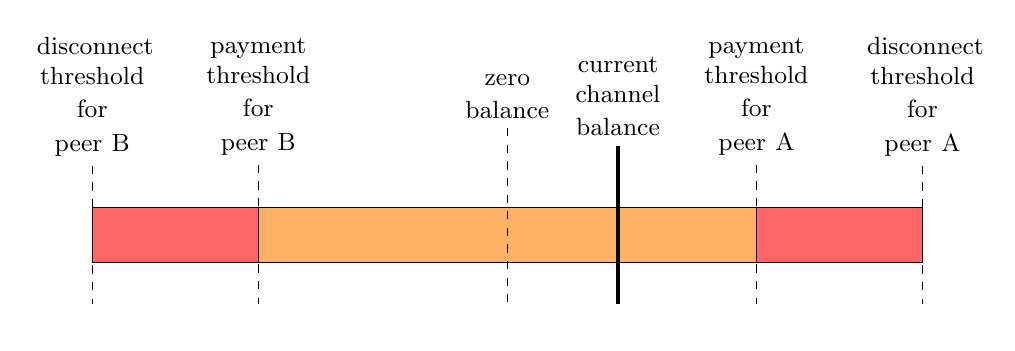
\begin{tikzpicture}
\node (middle)[draw, rectangle, fill=orange!60, minimum height=2em, minimum width=18em]{};
\node (leftred) [draw, rectangle, fill=red!60, minimum height=2em, minimum width=6em, node distance=12em,left of=middle]{};
\node (rightred)[draw, rectangle, fill=red!60, minimum height=2em, minimum width=6em, node distance=12em,right of=middle]{};
\node (zero) [above of=middle,node distance=5em, text width=4em, align=center] {\small zero\\ balance};
\node (zerod) [below of=middle] {};
\draw [dashed](zero)--(zerod);
\node (rtol) [node distance=9em,right of=zero,text width=4em, align=center] {\small payment\\threshold\\for peer A};
\node (rtold) [node distance=9em,right of=zerod] {};
\node (ltol) [node distance=9em,left of=zero,text width=4em, align=center] {\small payment\\threshold\\for peer B};
\node (ltold) [node distance=9em,left of=zerod] {};
\node (rdis) [node distance=15em, right of=zero,text width=4em, align=center] {\small disconnect\\threshold\\for peer A};
\node (rdisd) [node distance=15em,right of=zerod] {};
\node (ldis) [node distance=15em, left of=zero,text width=4em, align=center] {\small disconnect\\threshold\\for peer B};
\node (ldisd) [node distance=15em,left of=zerod] {};
\node (rbal) [node distance=4em,right of=zero,text width=4em, align=center] {\small current\\channel\\balance};
\node (rbald) [node distance=4em,right of=zerod] {};

\draw [dashed](rtol)--(rtold);
\draw [dashed](ltol)--(ltold);
\draw [dashed](rdis)--(rdisd);
\draw [dashed](ldis)--(ldisd);
\draw [very thick](rbal)--(rbald);
\end{tikzpicture}
\end{center}
\caption{Swap balance and swap thresholds.
Zero balance in the middle indicates consumption and provision are equal.
The current channel balance represents the difference in uncompensated service provision:
if to the right of zero, the balance tilts in favour of A with peer B being in debt, whereas to the left
the balance tilts in favour of B with A being in debt.
The orange interval represents loss tolerance. If the balance goes over the payment threshold, the party in
debt sends a cheque to its peer, if it reaches the disconnect threshold, the peer in debt is disconnected.}
\label{fig:swap}
\end{figure}
\end{center}

Swap also offers a way to deal with variance if extended with a delayed payment instrument
like the chequebook.
If the balance tilts too much toward one peer, the indebted
party issues a cheque to return the balance to zero.
This process is automatic and justifies swap as \emph{settle (the balance) with automated payments}
(see figure \ref{fig:swap}).

A valid cheque can always be directly cashed by sending it
in a transaction to the issuer's chequebook contract. Alternatively cheques can also be withheld.
Withholding a cheque is effectively lending on credit, which enables the parties to save on
transaction costs.
While, strictly speaking, there are no strong solvency guarantees,
a bounced cheque will affect the issuer's reputation (as the chequebook contract records it).
On the premise that
cheques are swapped in the context of repeating dealings, peers will refrain from
issuing cheques beyond their balance.
In other words, interest in keeping good reputation is a strong incentive for
solvency.

An additional advantage of this construct is that one can start providing service with zero ether.
Since swap can also work only one way, if a party enters the system with zero ether,
but connects to peers with a chequebook, they can provide service first to produce a positive balance.
If a node with funds connects to a peer without a contract, they tacitly agree to
create a chequebook contract for their peer in case they get indebted beyond
the amount needed for contract creation. Once a peer has their own chequebook contract, they are able
to consume and potentially pay out to the benefactor (see figure).
To summarise, by serving before consuming, participants can
bootstrap their way into swap without the need for funds.
Hence swap is justified as (\emph{setting up a wallet as payment}).

\begin{center}
\begin{figure}
\begin{center}
\begin{tabular}{ccc}
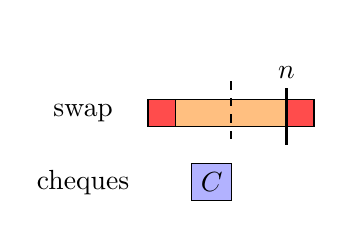
\begin{tikzpicture}
\node (middle)[draw, rectangle, fill=orange!50, minimum height=1em, minimum width=4em]{};
\node (leftred) [draw, rectangle, fill=red!70, minimum height=1em, minimum width=1em, node distance=2.5em, left of=middle]{};
\node (rightred)[draw, rectangle, fill=red!70, minimum height=1em, minimum width=1em, node distance=2.5em, right of=middle]{};
\node (zero) [above of=middle,node distance=2em, text height=1em] {};
\node (zerod) [below of=zero, node distance=3.5em] {};
\node (balance) [right of=zero,node distance=2em, text height=1.5em] {$n$};
\node (balanced) [below of=balance,node distance=3.5em] {};
\draw [dashed](zero)--(zerod);
\draw [very thick](balance)--(balanced);
\node (payment) [below of=zerod, node distance=1em]{};
\node (cheqeue) [draw, left of=payment, node distance=.7em, minimum height=1em, minimum width=1.4em, fill=blue!30, rectangle]{$C$};

\node (swap) [left of=leftred,minimum width=1em,align=right]{swap};
\node (cheques) [below of=swap,minimum width=1em, node distance= 2.5em, align=right]{cheques};
\end{tikzpicture}
&
\begin{tabular}{c}
  $\Longrightarrow$
\\ \\ \\ \\
\end{tabular}
&
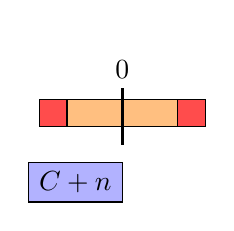
\begin{tikzpicture}
\node (middle)[draw, rectangle, fill=orange!50, minimum height=1em, minimum width=4em]{};
\node (leftred) [draw, rectangle, fill=red!70, minimum height=1em, minimum width=1em, node distance=2.5em, left of=middle]{};
\node (rightred)[draw, rectangle, fill=red!70, minimum height=1em, minimum width=1em, node distance=2.5em, right of=middle]{};
\node (zero) [above of=middle,node distance=2em, text height=1.5em] {$0$};
\node (zerod) [below of=zero, node distance=3.5em] {};
% \draw [dashed](zero)--(zerod);
\draw [very thick](zero)--(zerod);
\node (payment) [below of=zerod, node distance=1em]{};
\node (cheque) [draw, left of=payment, node distance=1.7em, minimum height=1em, minimum width=3.4em, fill=blue!30, rectangle]{$C+n$};
\end{tikzpicture}
\end{tabular}
\end{center}

\caption{Peer B's swap balance (with respect to A) reaches the payment threshold $n$ (left),
B sends a cheque to peer A. B keeps the cheque and restores the swap balance to zero.}
\label{fig:chequeswap}
\end{figure}
\end{center}

\subsection{Waivers}

If after a period of accumulating cheques the channel balance starts tilting the other way,
further savings are possible.
Assume peer A issued cheques to B and the balance was brought back to zero.
Now the balance tilts in A's favour but the cheques from A to B have not been cashed.
In this scenario, instead of sending a cheque to A, B can waive part of their entitlement.
This justifies swap as \emph{send waiver as payment} (see figure \ref{fig:waiverswap}).
A waiver essentially implements a proof that a cheque is destroyed, i.e., a promise
that (part of) an uncashed cheque will not be redeemed.

A \gls{waiver} is implemented as a note signed by the peer holding uncashed cheques.
The note specifies the current \gls{swap index} (sequential number) and
indicates the amount of dept they agree to waive from their entitlement.
If a channel is set to issue waived cheques then cashing must be a two step process.
Upon receiving a cheque, the contract verifies the signature and checks if
the swap index matches the one on the cheque.
If the cheque is valid, the claim amount is stored in a variable with a timestamp.
At this point a grace period starts: the original issuer gets notified of the cashing
request and is invited to send in their last (highest) waiver signed by their peer.

Analogously to cheques, waivers are accepted by the contract if sent in as data in
a transaction together with the issuer's address.
Upon receiving a waiver the contract verifies the signature and
checks if the swap index matches the one in the waiver.
If the waiver is valid, the peer's cumulative cashed balance is increased by the waived amount
pretending the waived amount was paid out. Then the new cumulative cashed balance is
compared to the one recorded when the cheque was received. Any remaining positive balance
is transfered to the beneficiary, the cumulative sum is cleared from storage and
the swap index is incremented.

During the grace period the amount is not checked against the book's global balance.
After the grace period expires and no waiver was received, a second transaction
increments the swap index and simply releases the funds or default on its debt.
During the grace period, further cheques can be sent to the contract: if they are valid
and have the same swap index as the one currently recorded, they simply replace
the earlier one and the grace period is renewed.
Since waivers need to match the swap index set by the cheques they destroy, they cannot
be sent to the contract before the cheque(s) they waive or after a new swap cycle starts.

In normal operation, however, peers are not incentivised to send in cheques as
long as they can issue waivers. Once the waiver goes over
the total amount of uncashed liabilities, the peer needs to send a cheque.
The swap index is incremented in this cheque and the basis for issuing is the channel
balance stored on the chain. This makes sure that cheques and
waivers cannot be reused.%
%
\footnote{The volume of cheques waived will not increase the cumulative balance and therefore
do not count toward total business volume for the purposes of credit history.
This can be amended if cheques are sent together with the latest waivers
and after validation the contract would adjust the cumulative balance to reflect the total volume.}

Using waivers can substantially increase the tolerated variance in the channel balance
without requiring actual transfer or impacting liquidity of the chequebook.
Without it, both peers would need to issue cheques and settlement would involve
transfering back and forth between the two peers, which means the first amount cashed
would not be available for a party for a period.

Waived cheques represent stronger guarantees since the cheque can effectively serve
as backing for incurring costs dedicated to the original issuer.

To summarise, Swap is ideally suited for immediately verifyiable, recurring micropayments for bidirectional
services. The primary usecase is bandwidth compensation and accounting to incentivise
relaying in a peer to peer system. As two peers are doing continuous business
they swap services, cheques and waivers and keep accounting and compensation offchain.




\begin{center}
\begin{figure}
\begin{center}
\begin{tabular}{ccc}
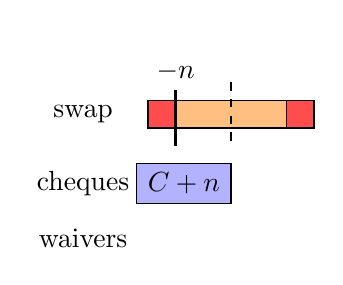
\begin{tikzpicture}
\node (middle)[draw, rectangle, fill=orange!50, minimum height=1em, minimum width=4em]{};
\node (leftred) [draw, rectangle, fill=red!70, minimum height=1em, minimum width=1em, node distance=2.5em, left of=middle]{};
\node (rightred)[draw, rectangle, fill=red!70, minimum height=1em, minimum width=1em, node distance=2.5em, right of=middle]{};
\node (zero) [above of=middle,node distance=2em, text height=1em] {};
\node (zerod) [below of=zero, node distance=3.5em] {};
\node (balance) [left of=zero,node distance=2em, text height=1.5em] {$-n$};
\node (balanced) [below of=balance,node distance=3.5em] {};
\draw [dashed](zero)--(zerod);
\draw [very thick](balance)--(balanced);
\node (payment) [below of=zerod, node distance=1em]{};
\node (cheque) [draw, left of=payment, node distance=1.7em, minimum height=1em, minimum width=3.4em, fill=blue!30, rectangle]{$C+n$};

\node (swap) [left of=leftred,minimum width=1em,align=right]{swap};
\node (cheques) [below of=swap,minimum width=1em, node distance= 2.5em, align=right]{cheques};
\node (waivers) [below of=cheques,minimum width=1em, node distance= 2em, align=right]{waivers};
\end{tikzpicture}
&
\begin{tabular}{c}
  $\Longrightarrow$
\\ \\ \\ \\
\end{tabular}
&
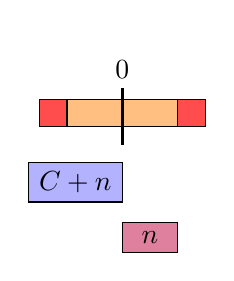
\begin{tikzpicture}
\node (middle)[draw, rectangle, fill=orange!50, minimum height=1em, minimum width=4em]{};
\node (leftred) [draw, rectangle, fill=red!70, minimum height=1em, minimum width=1em, node distance=2.5em, left of=middle]{};
\node (rightred)[draw, rectangle, fill=red!70, minimum height=1em, minimum width=1em, node distance=2.5em, right of=middle]{};
\node (zero) [above of=middle,node distance=2em, text height=1.5em] {$0$};
\node (zerod) [below of=zero, node distance=3.5em] {};
% \draw [dashed](zero)--(zerod);
\draw [very thick](zero)--(zerod);
\node (payment) [below of=zerod, node distance=1em]{};
\node (cheque) [draw, left of=payment, node distance=1.7em, minimum height=1em, minimum width=3.4em, fill=blue!30, rectangle]{$C+n$};
\node (waivers) [below of=payment, node distance=2em]{};
\node (waiver) [right of=waivers,minimum width=2em, node distance=1em,rectangle,draw,fill=purple!50]{$n$};
\end{tikzpicture}
\end{tabular}
\end{center}

\caption{Peer A's swap balance (with respect to B) reaches the payment threshold $n$ (left),
A sends a waiver to peer B. B keeps the waiver and restores the swap balance to zero}
\label{fig:waiverswap}
\end{figure}
\end{center}

\subsection{Payment channels}

If the variance is expected to be higher than the loss a peer can afford,
risk of insolvency can be mitigated by assigning part of the balance to a beneficiary.
This locked up sum, called \gls{channel deposit} allows the owner a tilted balance and
serves as assured collateral dedicated to a particular peer.
This can be implemented by keeping peer-specific balances in the chequebook contract.
This deposit is no longer pooled over multiple creditors
and locking it can guarantee successful cashing of cheques up to the deposited amount.
Withdrawal from the channel deposit is possible but involves a grace period during which
the counterparty is invited to challange the current balance by sending in the (last) cheque
with the highest amount. After the grace period the owner can reduce the deposit to cover only
its actual debt and may withdraw the remainder.
In order to get the balance of account between peers, the contract needs access to the counterparty
chequebook contract. For ease of explanation we assume that beneficiary is the
chequebook contract itself. Channel deposits can then be implemented as a map with beneficiary contract
address as key and the integer balance in wei as value.

Two chequebook contracts that have a record for each other constitute what is
called a \gls{payment channel}.


\begin{center}
\begin{figure}
\begin{center}
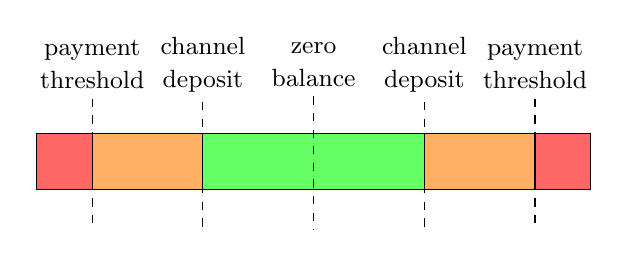
\begin{tikzpicture}
  \node (middle)[draw, rectangle, fill=green!60, minimum height=2em, minimum width=8em]{};
  \node (midleft)[draw, rectangle, fill=orange!60, minimum height=2em, minimum width=4em, node distance=6em, left of=middle]{};
\node (midright)[draw, rectangle, fill=orange!60, minimum height=2em, minimum width=4em, node distance=6em, right of=middle]{};
\node (leftred) [draw, rectangle, fill=red!60, minimum height=2em, minimum width=2em, node distance=9em,left of=middle]{};
\node (rightred)[draw, rectangle, fill=red!60, minimum height=2em, minimum width=2em, node distance=9em,right of=middle]{};
\node (zero) [above of=middle,node distance=3.5em, text width=4em, align=center] {\small zero\\ balance};
\node (zerod) [below of=middle] {};
\draw [dashed](zero)--(zerod);
\node (rtol) [node distance=8em,right of=zero,text width=4em, align=center] {\small payment\\threshold};
\node (rtold) [node distance=8em,right of=zerod] {};
\node (ltol) [node distance=8em,left of=zero,text width=4em, align=center] {\small payment\\threshold};
\node (ltold) [node distance=8em,left of=zerod] {};
\node (prtol) [node distance=4em,right of=zero,text width=4em, align=center] {\small channel\\deposit};
\node (prtold) [node distance=4em,right of=zerod] {};
\node (pltol) [node distance=4em,left of=zero,text width=4em, align=center] {\small channel\\deposit};
\node (pltold) [node distance=4em,left of=zerod] {};
\draw [dashed](rtol)--(rtold);
\draw [dashed](ltol)--(ltold);
\draw [dashed](prtol)--(prtold);
\draw [dashed](pltol)--(pltold);
\end{tikzpicture}
\end{center}
\caption{}
\label{fig:paymentchannel}
\end{figure}
\end{center}


\section{Escrow conditions on future payments}

\gls{Promissory notes} represent redeemable promises of payment potentially maturing in the future.
We define the general notion of a note as a promise that entitles a beneficiary to future payment
under a condition. Since this effectively puts the money in an escrow, the condition can
also be referred to as an \gls{escrow condition}.
A promissory note can contain the following optional fields:

  \begin{itemize}
    \item amount
    \item beneficiary
    \item escrow address
    \item valid from
    \item valid until
    \item swap index
  \end{itemize}

In the simplest case no escrow condition or maturation date is given: such a note
represents a simple cheque as discussed above.
The maturation date (blockheight or timestamp) can be specified to indicate the earliest
possible occasion a note can be redeemed (valid from) as well as a deadline when the promise
expires unless its escrow condition is satisfied (valid until).

\subsection{Recurring payments}

The cheque represents an adhoc promise to redeem an amount.
The transfer of funds is sanctioned by a cheque issued for each occasion.
There is, however, services where recurring payments are predictable and therefore
the installments can be sanctioned in advance. The primary usecase is subscription
services.
This could be implemented by storing a whitelist of contract addresses that are allowed
to withdraw from the chequebook balance.
For simplicity, however, we choose to represent this analogously to cashing a cheque.
Authorising a recurring payment to a contract is done by signing a blank cheque (a cheque with
an unspecified amount) against the beneficiary possibly with a valid until date.
Such beneficiaries are smart contracts and therefore no defense against
false amount is needed.
Receiving transfer request transactions is independent of the swap state of cumulative amount
and simply withdraws the amount from the global balance or the channel deposit of the owner.

\subsection{Bonds}

A note with an amount and beneficiary and a future valid from data is effectively a bond.
The amount factors in all outstanding payment obligations the beneficiary is entitled to
once the bond matures including interest. When such a note is not collateralised at the time of issuing,
accepting the bond is equivalent to granting a loan on the grounds of the credit history of the account.

\subsection{Escrow conditions and escrow witnesses}

If an escrow address is specified in the note, the referenced contract can be used to verify the condition
of redemption. When the escrow condition is verified, the owner, the beneficiary address, and
the note id (the hash of the signed note) are passed as arguments to the {\gls{testimonyFor?}} method
of the escrow contract. By implementing this method the contract conforms to the \gls{witness} contract
 interface
(section \ref{sec:courtroom}). Given the witness contract, the escrow condition is implicitly defined
as whatever state makes the escrow witness give a positive testimony.

A note with an escrow field specified is called a \gls{conditional bond} and
can represent a \gls{service contract} with the escrow condition describing successful delivery.
In a real-life scenario, upon verification of an instance of service provision or purchase of a good,
the escrow acknowledges the delivery before releasing the funds.
This is implemented by the chequebook calling the escrow witness contract
to give a testimony. In case the condition is fully verifiable algorithmically in the VM,
the entire transaction remains within the closed system, there is no real-world liability and the transfer
is enforcable.

If no beneficiary is specified, a conditional note is essentially a \gls{bounty}.
A bounty is meant to be published or broadcast to a set of known service providers.
Figure \ref{fig:taxonomy} summarises the various types of promissory notes.


\newcommand{\tick}{$X$}
\newcommand{\opt}{$(X)$}
\begin{center}
\begin{figure}
\begin{center}
\begin{tabular}{|l||c|c|c|c|c|c|}
\hline
\multicolumn{1}{|c||}{type}
& \multicolumn{6}{c|}{fields}
\\
\cline{2-7}
& swap index
& amount
& beneficiary
& escrow
& valid from
& valid until
\\
\hline
\hline
cheque & \tick & \tick & \tick & & & \opt
\\
authorisation &  & \tick & \tick & & & \opt
\\
bond & \tick & \tick & \tick & & \tick & \opt
\\
conditional bond &  & \tick & \tick & \tick & \opt & \opt
\\
bounty & \tick &  \tick & & \tick & \opt & \opt
\\
soft channel deposit &  \tick & \tick & & & &
\\
\hline
\end{tabular}
\end{center}
\caption{Taxonomy of promissory notes}
\label{fig:taxonomy}
\end{figure}
\end{center}


% \subsection{Secure escrow and liquidity}

\subsection{Conditional bond, invoice, and cheque}

Let us assume that node A issues a conditional note (or bounty) to B with expiry at time T.
T represents the earliest time that A can consider the note unfulfilled (the service undelivered), before
that we say that the note is \emph{active}.

If B fulfills the condition, it notifies A of successful delivery
by sending an \gls{invoice} containing the hash of the note and the current cumulative balance they want the
amount to be added to. The invoice is supposed to represent the balance at delivery, and serves to
indicate that the subsequent cheque will be the one to pay the outstanding amount for the note.
As a response A is expected to send a cheque with an updated channel balance reflecting the
payment of the invoice (the amount in the conditional note is added to the cumulative total).
If A refuses to do this, B can send the conditional note in a transaction
to  the contract. When the witness validates the delivery condition, and the testimony is
positive, the amount goes to escrow and a grace period starts.
During the grace period, A can settle the claim by sending in the appropriate cheque.

If the note condition does not check out, B's challenge will cost them the transaction.
Even if it does, they won't gain anything by the challange if they did receive the
cheque from A since they still needed to send the proof in a transaction.
Therefore B is disincentived to initiate frivolous challenges.
Conversely, A is incentivised to send the cheque to B after it receives the invoice,
otherwise it is A that needs to pay transaction cost of sending in the cheque upon B's correct challenge.
We therefore conclude that the optimal behaviour for A and B is offchain exchange of invoice and cheque.

\subsection{Soft channel deposits}
A nonmaturing cheque is a deposit locked up as collateral to secure varying balance.
The total value of these deposits serve as guaranteed collateral for any debt and
therefore conceptually equivalent to a channel deposit.
In the following we describe a construct which gives 100$\%$ guarantee of solvency
on outstanding conditional bonds without explicitly assigning deposits to channels on chain.%
%
\footnote{In the on-chain case channel deposits are explicitly stored in the contract, therefore overspending
(using the amount to collateralise multiple creditors) is impossible.}

Let us assume A and B both maintain an ordered list of active conditional notes issued by A.
Each time A issues a conditional note or pays for a fulfilled one or one expires, the list is updated.
The hashes of active notes in order of issueance is organised in a swarm tree, the
root hash of which is signed by B and passed to A together with a so called
\gls{soft channel deposit claim}. This claim constitutes an acknowledment of
the outstanding liabilities of A towards B. Assume further that there exist a notion of \gls{epoch},
a fixed settlement period at the end of which B needs to sign off on the total sum of active
outstanding conditional notes issued by A to B.
Formally, soft channel deposit claim is a note with the following fields:

\begin{itemize}
  \item A's contract address
  \item the total sum of all active outstanding conditional notes
  \item the epoch index
\end{itemize}

With each epoch, B signs the note and sends it to A.
Peer A can verify if the soft claim is correct and terminate dealings if not. In such a case soft claim of
the last epoch is taken, whereby A cancels its liability to the conditional notes issued since
the last epoch.
B is incentivised to send the correct soft claim if they want business with A fulfilling their
conditional notes.

After A receives soft channel deposit claims from all peers for the epoch, the claims are
collected in a list (ordered according to the peer index of the beneficiary in A's swap contract).
A signs the swarm hash of the (concatenated) list and sends it alongside the list
in a construct called a \gls{soft channel deposit allocation table} to each peer.
Upon receiving the soft channel deposit allocation table, B verifies that
(1) the total sum of channel deposits allocated is no greater than the global deposit and
(2) the amount dedicated to B is no less than the sum of all outstanding active
conditional notes issued by A to B.
(3) each active peer in A's swap contract has a corresponding claim for the current epoch and the signature is valid.

At any point in time, soft channel deposit claims can be consolidated to actual
channel deposits.
The soft channel deposit claim is sent in with the inclusion proof of the claim against the root hash of the
current channel deposit allocation table as a transaction to the
chequebook contract. Upon receiving and validating the claim (signature, resource and epoch verified),
the contract simply reallocates the claimed amount from the global deposit to the channel.
If each peer does this, the global deposit is reduced with the total of soft channel
deposits.%
%
\footnote{To save all peers the trouble of sending inclusion proofs, when A initiates withdrawal from
their global deposit, they need to submit the actual allocation table starting a grace period during which
creditors are invited to challenge the allocation by presenting a contradicting claim.}

Once the channel deposit (of A towards B) is secured on chain, all the outstanding conditional notes
issued to B are guaranteed to be redeemable in the standard ways.
If a peer is found to issue contradictory channel claims for the same epoch, they relinquish
their right to any claim. For any third party this entails that if a peer's claim is
included in the allocation table, the maximum they are entitled to redeem is limited:
(1) the sum in the claim if they signed a correct unique claim or
(2) zero if they illegally signed multiple claims for the same epoch.
Futhermore, since the allocation table is exhaustive, i.e., each
peer signed their claim, third parties can also assume that the sum of all claims in the
allocation table is the maximum total deposit that can be consolidated.

If the soft channel deposit allocation table is valid,
we can with complete certainty know that the global deposit in A's contract
 could cover all outstanding conditional notes handed to B even if all peers were to redeem all outstanding notes.
Practically this means then that, after receiving a valid allocation table for the epoch from A,
B has no risk of insolvency when dealing with A's conditional notes.

In sum, using soft channel deposits enables the chequebook owner to allocate and reallocate funds
as channel deposits in a fairly flexible way without blockchain transaction costs,
yet provide $100\%$ solvency guarantees on all active conditional bonds to their peers.


\section{Service guarantees}

\subsection{Service guarantees}
\label{sec:courtroom}

In the previous section we introduced tools to compensate service providers.
While rewards are paid out only if delivery is successful,
such positive incentivisation may be insufficient if
explicit guarantees of future delivery are required.

In this section we describe a system of service contracts and dispute resolution.
Service contracts allow providers (or a set of providers)
to offer quality and/or delivery guarantees to customers.
Without loss of generality, we can conceptualise a service contract as a contract
on the blockchain.
Nodes can commit to a service contract by registering their address in the contract
with a transaction or issuing a signed note offchain.
By committing to this specification providers can be held accountable for non-compliance.

Litigation on the other hand, allows customers to initiate an on-chain court procedure
in case they suspect foul play. Such accountability is
crucial for the design of scalable decentralised service economies.

We will describe the trial process for dispute
resolution that first evaluates the evidence agaist the accused provider.
The verification is the same as the one used in the process of sanctioning outpayments,
but once a provider is proven guilty by the court on the grounds of
conditions specified in the service contract, various punitive measures will be
automatically enforced. In most cases, this comprises losing some deposit that
provider previously locked up as collateral to back their promise.%
%
\footnote{Instead of or in addition to losing their deposits, nodes would also
suffer loss of reputation. If any demonstrated violation of terms is
recorded on the public blockchain, users can expect clean histories as a measure
of reputation.}
%

By registering on a service contract and putting up a deposit if required, providers
swear to play by the rules.
This deposit is locked up and used later as compensatory insurance transfered to the
customer, redistributed or burnt.


\subsection{Conducting a trial}

If a service provider is suspected of non-compliance, they can be challenged
by opening a case with the swear contract.
An abstract trial is composed of stages of litigation, at each stage
the court procedure calls witnesses and depending on their testimony
advance the trial into the next stage. Witnesses can refuse testimony
if evidence is not (yet) available in which case the trial
is paused until the grace period allowed to submit evidence is over.
Eventually the trial concludes with a guilty or not guilty verdict followed
by automatically enforced punitive measures in the former case or
compensation to the accused in the latter.

The specific service contract describes the rules of the service
by assigning particular expert witnesses to trial stages. These witnesses
evaluate evidence submitted to them in relation to the case
and give testimony if asked by the judge.
The request--response process between the judge and the witnesses can
thus be standardized
even though they each may require different data to be submitted to them as evidence.

To implement such an abstract dispute resolution system
the trial is described by a finite state automaton the states of which correspond
to stages of litigation and
the transitions are labeled by various outcomes of evaluating evidence submitted
to the respective expert witness associated with the stage. A witness
is a smart contract that implements the $\mathit{testimonyFor}$ function which takes
as arguments the provider address, the plaintiff address, and the note id (the hash of the signed note)
representing the service request.
The \gls{swindle} contract orchestrates the transition through the stages calling the witness contracts,
handles grace periods to control the deadline for submitting evidence (challenges or their refutations) to
eventually reach a guilty/non-guilty verdict on the grounds of witness testimonies.
In case of a guilty verdict, the deposit sworn on is forfeited and the peer's registration is
terminated.

\begin{center}
\begin{figure}
\begin{center}
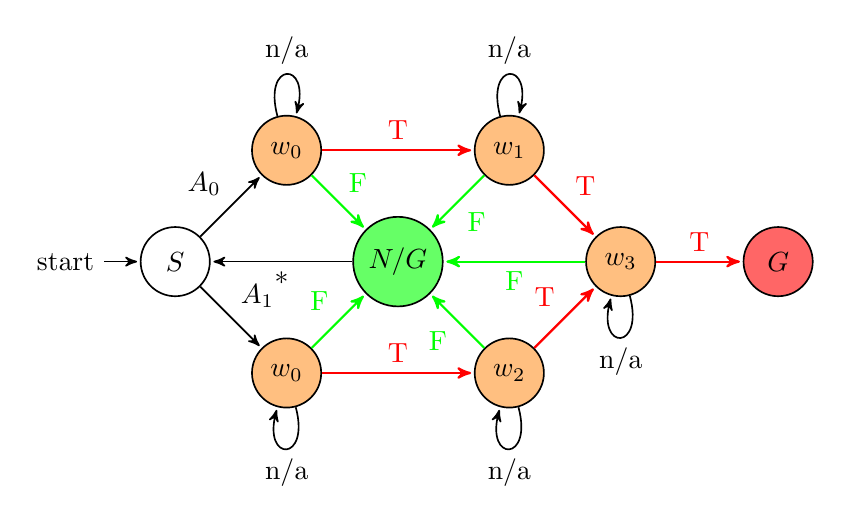
\begin{tikzpicture}[->,>=stealth',shorten >=1pt,auto,node distance=2c m,
                    semithick]
  \tikzstyle{witness}=[fill=orange!50,draw]
  % \tikzstyle{every state}=[fill=gray!10,draw]

  \node[initial,state] (S)                    {$S$};
  \node[state,witness]         (W0_1) [above right of=S] {$w_0$};
  \node[state,witness]         (W0_2) [below right of=S] {$w_0$};
  \node[state,fill=green!60]         (N/G) [below right of=W0_1] {$N/G$};
  \node[state,witness]         (W1) [above right of=N/G] {$w_1$};
  \node[state,witness]         (W2) [below right of=N/G] {$w_2$};
  \node[state,witness]         (W3) [below right of=W1] {$w_3$};
  \node[state,fill=red!60]         (G) [right of=W3]       {$G$};

  \path (S) edge   node {$A_0$} (W0_1)
            edge   node {$A_1$} (W0_2)
        (W0_1) edge [loop above] node {n/a} (W0_1)
            edge [red,thick]             node {T} (W1)
            edge [green,thick]             node {F} (N/G)
        (W0_2) edge [loop below] node {n/a} (W0_2)
            edge [red,thick]             node {T} (W2)
            edge [green,thick]             node {F} (N/G)
        (W1) edge [loop above] node {n/a} (W1)
            edge [red,thick]             node {T} (W3)
            edge [green,thick]             node {F} (N/G)
        (W2) edge [loop below] node {n/a} (W2)
            edge  [red,thick]            node {T} (W3)
            edge  [green,thick]            node {F} (N/G)
        (N/G) edge              node {*} (S)
        (W3) edge [loop below] node {n/a} (W3)
            edge  [green,thick]            node {F} (N/G)
            edge [red,thick]  node {T} (G);
\end{tikzpicture}
\end{center}
\caption{Trial stages represented as a finite state automaton describing a service contract.
Upon receiving an accusation ($A_0$ or $A_1$) in a transaction, the case contract moves to the first litigation state.
The orange circles represent states where a witness contract is called, the following state depends on
the outcome of the witness testimony (the return value of the $\mathit{testimonyFor}$ function call).
The other nodes call the internal $\mathit{process}$ function: to pay compensation if the challenge is refuted (N/G) or enforce
the sentence in case of a guilty verdict (G).}
\label{fig:servicecontract}
\end{figure}
\end{center}


\section{Service networks}

In this section we describe how the tools for peer-to-peer accounting and data-exchange can
be used to drive the incentives for distributed digital services.
Assume that a set of nodes form a network that provides a decentalised service.
Insured chunk storage in swarm, arbitrary remote payments or database insertion are examples of such services.
A \gls{service task} is defined as an instance of service provision. Storing a particular chunk, paying
an amount to another node or inserting an entry to an index are examples of tasks of the respective network
service.

In what follows we will work with the assumption that the participating nodes in a service network are
connected in a kademlia topology and can relay messages to other nodes using kademlia deterministic routing
based on direct devp2p transport layer for each hop. In other words service networks are composed of a subset
of nodes within swarm.

Scalability of
swap channels is based on the premise that directly connected nodes engage in long-term repeated
dealings and can afford setting up contracts on the blockchain to secure their interaction.%
%
\footnote{Given the semipermanent connections of the TCP based kademlia of swarm, peers interact with
$O(log(n))$ peers where $n$ is the number of nodes in the network.}
%
Service networks enable \gls{indirect transactions} by relaying tasks and deliveries using
swap-channel transactions on every hop.
This makes it possible to preserve the scalability and security
of swap yet extend the scope of transactions both in terms of
frequency and reach, i.e., enabling \emph{ad-hoc one-off interactions between any two nodes}.
Service networks with global provision guarantees further improve the scope by
offering guaranteed market making and delivery in a direct immediately settling
swap transaction. As a result non-participating users can just \emph{request and disappear}.

\subsection{Incentivisation for relaying}

Let's assume that nodes A,B,C,D are participant peers of a service network such that
A-B, B-C and C-D are direct connections with a swap channel.
Assume further that A intends to do some ad-hoc one-off business with D. To this end
 A issues a conditional bond specifying an escrow
condition that some data be obtained from D constituting the proof of delivery of the task.

A then sends the conditional bond to B as beneficiary, B receives the conditional bond
and issues the same bond
only this time with C as beneficiary. C is directly connected to D, so
it just relays the same to D who issues a receipt (or takeover proof).
Each of these steps is implemented as swaps of conditional notes. The moment C receives
the receipt, it is incentivised to pass it back to B as an invoice to prompt
settlement. The same is true for B and any number of intermediate relaying nodes
(see figure \ref{fig:swapchannelnetwork}).

In general, we define an \emph{indirect transaction} as a chain of swaps between directly connected
peers. The success of a such indirect transactions between two nodes is dependent on whether and
how such a chain can be found. Our assumption is that the nodes have semipermanent connectivity
and form a network topology where routing between any two nodes is guaranteed, e.g., kademlia.

In order to incentivise relaying nodes to take part in such a network,
a transaction fee for every hop needs to be introduced.  We stipulate that the transaction fee
for one swap is proportional to the logarighmic distance that the hop spans.
As a consequence, the simple rational strategy to maximise profit will incentivise nodes to find the
closest node when relaying as well as maintain a healthy connectivity that is the
prerequisite for successful routing.
Furthermore, the entire transaction fee can be precalculated as proportional
to the distance between sender and remote beneficiary and therefore can be offered in advance
when issuing the conditional bond.

This construct is
equivalent to message relaying with \gls{certified delivery}, except that nodes are required to have
funds to cover the amount of the conditional bond.
For live connections in a service network to be operational,
parties agree to always having in-channel capacity in the amount of X.
With soft channel deposits, such throughput restrictions can easily
be mitigated even on an on-demand basis.

In addition to swap channels, connected nodes can maintain a \gls{provable data exchange}.
Assume that two nodes participate in a particular service that involve
relaying objects (such as requests and responses).
The content addresses (swarm hash) of consecutive objects
sent one direction constitute a \emph{data stream}.
Both peers save this stream to swarm and maintain an index mapping the hashes to offsets.
The upstream peer (sender) calculates the swarm hash of this index and periodically
signs it against the current blockheight or timestamp as well as the channel id.
This \gls{handover state} is periodically sent to the downstream peer (receiver)
who verifies it and preserves it until the next one.
Downstream peer periodically countersigns the handover state together with an initial
offset or timestamp. This \gls{takeover state} is then sent to the upstream peer.
For instance, the handover state obtained from the upstream peer can be used to prove to third parties
that an object X was handed over to the downstream peer. This can be done by
giving an inclusion proof of the hash of X.%
%
\footnote{Upstream peer can be challenged to give an inclusion proof.}

On top of the rewards peers get for relaying, we can introduce additional
incentives to guarantee that messages reach the recipient.
If nodes have a stake to lose, punitive measures can be imposed on non-relaying nodes.
If relaying nodes register on a service contract they promise to relay messages in a data stream
towards the recipient.

Take our earlier example of A sending a message to remote node D, and assume that
B, C, and D are all registered relaying nodes that are online. If there is reason
to believe that the message did not reach D, A can challange B by simply providing
the takeover proof for the message. B can defend itself by providing takeover proof from C,
thereby shifting the blame to C for blocking the delivery. C in turn can show takeover proof
from D to refute the challenge. It can also happen that C indeed did not forward the message
because there was no nodes closer to D among its peers. But this means that
D is a nearest neighbour of C, in which case D should have been connected to C.
Therefore D can be challenged to prove that it was connected to C. D can respond to the challenge
by showing handover state obtained from C dated after the message delivery deadline. This in turn is
a challenge to C to show the inclusion proof of the message against the handover state.
This pattern is called \gls{finger pointing} and constitutes the investigative part
of litigation which results in identifying the node
ultimately responsible for failed delivery by not relaying.
Finger pointing essentially implements \emph{guaranteed delivery}.

\subsection{Uniform resource allocation and market making}

In the previous section we just assumed that A knew about D (from an independent source).
In case there are other nodes as well that can in theory perform the same task,
a bounty is sent to potentially multiple addresses of candidate providers
and an implicit market making mechanism is obtained by certified delivery.

Assume the tasks of a service network can be provided by any participating node using
the same amount of resources. Given a network of willing providers, a system can be designed
called \gls{global resource allocation by network topology (GRANT)}
such that tasks are distributed more or less uniformly across the network.

For instance, this is the case with storage in swarm:
each task of storage provision involves storing a fixed-size chunk of data.
We index the chunks with their content address (swarm hash) and allocate the storage task
to nodes whose address is closest to the chunk address.
Since both nodes and chunks are uniformly distributed in the same address space,
this strategy implements uniform load balancing. We can generalise this allocation
strategy for any task if requirements
are uniform across tasks by simply indexing the task requests with their hash.

When a service user issues a bounty to request a service task, the bounty
is sent towards its address using kademlia routing.
If hops use provable data streams, the incentives can make sure
that the appropriate nodes are granted the provision of the task.

This node is dynamically defined as the closest node at any point in time.
For continuous services such as chunk storage, this means that as nodes leave
and join the network, the node responsible can change over time.
With data exchange proofs however, we can enforce that nodes synchronise historical
tasks and therefore the allocation can be taken for granted, i.e., the network
can perform dynamic load-balancing of previously submitted future tasks even though
the network is changing.

In order to benefit from the allocated tasks by cashing the bounties, the distribution
should be incentivised. In particular relaying nodes are not supposed to withhold
tasks in hope of cashing the bounty themselves.
To guarantee that downstream peers do get forwarded all the tasks and bounties,
upstream peers can be challenged when they cash a bounty:
if there is a valid handover proof of connection (synchronisation)
for the relevant period after the bond was issued, upstream peer can be challanged
for not relaying it (but withholding). Conversely, the bounty outpayment can be challenged
if the candidate provider is not the closest node to the task, i.e., a downstream peer closer to
the task address can show connectivity during the relevant period. Withholding if proven could
result in the same punitive measure as failing to deliver.


Service nodes that are capable staying online can choose to register
and put up a deposit as collateral.
One consequence of GRANT is that for each task, there is a node (or set of neighbouring nodes)
that is responsible for delivering the task and can ultimately be held liable
for non-delivery. Using the swindle scheme for litigation, if proven guilty node's
collateral is forfeited.
Since individual punitive measures are a very
effective incentive, service guarantees can be given independent of the
positive incentivisation (the reward for delivery implicit in the bounty).%
%
\footnote{Since the amount of tasks (and therefore capacity requirements) are roughly uniform for each
participant node, catastrophic failure of an entire node can cause limited damage.
Since the required deposit is meant to collateralise this risk, it is reasonable to
set it to a fixed amount across all provider nodes.}

When the issuer receives the receipt for its bounty (takeover proof or receipt)
it has all it is needed to start finger pointing which is equivalent to
instant guarantees that the service will be provided,
even though it is unknown at the time by which node.

This type of service network is called \gls{warranted automatic service provision (WASP)} network.
Since one can thus obtain enforcable service contracts immediately
in one swap exchange, WASP networks allow users to \emph{request and disappear}.

\section{Pricing in service networks}

The problem of pricing appears already when we

\subsection{Reverse auction for competitive bounties}
\subsection{Signalling capacity overload}
\subsection{Service networks for stablecoins}

\cite{btcmicro2014}
\cite{decker2015fast}
\cite{poon2015bitcoin}  %lightnening
\cite{prihodko2016flare} % routing in lightening
\cite{tremback2015universal}  %paymentchannels
\cite{bonneau2014mixcoin} % anonimity
\cite{ethersphere2016sw3}
\cite{ethersphere2016smash}
\cite{maymounkov2002kademlia}
\cite{heep2010r}
\cite{malavolta2017concurrency}
\cite{chiesa2017decentralized}
\cite{heilman2016tumblebit}
\cite{green2016bolt}
\cite{miller2017sprites}
\cite{mcdonald2017payment}
\cite{diferrante2017payment}

\bibliography{../refs.bib}
\appendix
\section{Swap contract}
\section{Swear and swindle contract}
\section{Swarm storage insurance}
\section{Scalable node-to-node payments}
\printglossary

\end{document}
